
%% bare_conf.tex
%% V1.3
%% 2007/01/11
%% by Michael Shell
%% See:
%% http://www.michaelshell.org/
%% for current contact information.
%%
%% This is a skeleton file demonstrating the use of IEEEtran.cls
%% (requires IEEEtran.cls version 1.7 or later) with an IEEE conference paper.
%%
%% Support sites:
%% http://www.michaelshell.org/tex/ieeetran/
%% http://www.ctan.org/tex-archive/macros/latex/contrib/IEEEtran/
%% and
%% http://www.ieee.org/

%%*************************************************************************
%% Legal Notice:
%% This code is offered as-is without any warranty either expressed or
%% implied; without even the implied warranty of MERCHANTABILITY or
%% FITNESS FOR A PARTICULAR PURPOSE! 
%% User assumes all risk.
%% In no event shall IEEE or any contributor to this code be liable for
%% any damages or losses, including, but not limited to, incidental,
%% consequential, or any other damages, resulting from the use or misuse
%% of any information contained here.
%%
%% All comments are the opinions of their respective authors and are not
%% necessarily endorsed by the IEEE.
%%
%% This work is distributed under the LaTeX Project Public License (LPPL)
%% ( http://www.latex-project.org/ ) version 1.3, and may be freely used,
%% distributed and modified. A copy of the LPPL, version 1.3, is included
%% in the base LaTeX documentation of all distributions of LaTeX released
%% 2003/12/01 or later.
%% Retain all contribution notices and credits.
%% ** Modified files should be clearly indicated as such, including  **
%% ** renaming them and changing author support contact information. **
%%
%% File list of work: IEEEtran.cls, IEEEtran_HOWTO.pdf, bare_adv.tex,
%%                    bare_conf.tex, bare_jrnl.tex, bare_jrnl_compsoc.tex
%%*************************************************************************

% *** Authors should verify (and, if needed, correct) their LaTeX system  ***
% *** with the testflow diagnostic prior to trusting their LaTeX platform ***
% *** with production work. IEEE's font choices can trigger bugs that do  ***
% *** not appear when using other class files.                            ***
% The testflow support page is at:
% http://www.michaelshell.org/tex/testflow/



% Note that the a4paper option is mainly intended so that authors in
% countries using A4 can easily print to A4 and see how their papers will
% look in print - the typesetting of the document will not typically be
% affected with changes in paper size (but the bottom and side margins will).
% Use the testflow package mentioned above to verify correct handling of
% both paper sizes by the user's LaTeX system.
%
% Also note that the "draftcls" or "draftclsnofoot", not "draft", option
% should be used if it is desired that the figures are to be displayed in
% draft mode.
%
\documentclass[10pt, conference, compsocconf]{IEEEtran}
% Add the compsocconf option for Computer Society conferences.
%
% If IEEEtran.cls has not been installed into the LaTeX system files,
% manually specify the path to it like:
% \documentclass[conference]{../sty/IEEEtran}





% Some very useful LaTeX packages include:
% (uncomment the ones you want to load)


% *** MISC UTILITY PACKAGES ***
%
%\usepackage{ifpdf}
% Heiko Oberdiek's ifpdf.sty is very useful if you need conditional
% compilation based on whether the output is pdf or dvi.
% usage:
% \ifpdf
%   % pdf code
% \else
%   % dvi code
% \fi
% The latest version of ifpdf.sty can be obtained from:
% http://www.ctan.org/tex-archive/macros/latex/contrib/oberdiek/
% Also, note that IEEEtran.cls V1.7 and later provides a builtin
% \ifCLASSINFOpdf conditional that works the same way.
% When switching from latex to pdflatex and vice-versa, the compiler may
% have to be run twice to clear warning/error messages.






% *** CITATION PACKAGES ***
%
\usepackage{cite}
\usepackage{textcomp}
\usepackage{xcolor}
\usepackage{multirow}
%\def\BibTeX{{\rm B\kern-.05em{\sc i\kern-.025em b}\kern-.08em
 %   T\kern-.1667em\lower.7ex\hbox{E}\kern-.125emX}}
% cite.sty was written by Donald Arseneau
% V1.6 and later of IEEEtran pre-defines the format of the cite.sty package
% \cite{} output to follow that of IEEE. Loading the cite package will
% result in citation numbers being automatically sorted and properly
% "compressed/ranged". e.g., [1], [9], [2], [7], [5], [6] without using
% cite.sty will become [1], [2], [5]--[7], [9] using cite.sty. cite.sty's
% \cite will automatically add leading space, if needed. Use cite.sty's
% noadjust option (cite.sty V3.8 and later) if you want to turn this off.
% cite.sty is already installed on most LaTeX systems. Be sure and use
% version 4.0 (2003-05-27) and later if using hyperref.sty. cite.sty does
% not currently provide for hyperlinked citations.
% The latest version can be obtained at:
% http://www.ctan.org/tex-archive/macros/latex/contrib/cite/
% The documentation is contained in the cite.sty file itself.






% *** GRAPHICS RELATED PACKAGES ***
%
\ifCLASSINFOpdf
  \usepackage[pdftex]{graphicx}
  % declare the path(s) where your graphic files are
  \graphicspath{{../}}
  % and their extensions so you won't have to specify these with
  % every instance of \includegraphics
  \DeclareGraphicsExtensions{.pdf,.jpeg,.png}
\else
  % or other class option (dvipsone, dvipdf, if not using dvips). graphicx
  % will default to the driver specified in the system graphics.cfg if no
  % driver is specified.
  \usepackage[dvips]{graphicx}
  % declare the path(s) where your graphic files are
  \graphicspath{{../}}
  % and their extensions so you won't have to specify these with
  % every instance of \includegraphics
  \DeclareGraphicsExtensions{.eps}
\fi
% graphicx was written by David Carlisle and Sebastian Rahtz. It is
% required if you want graphics, photos, etc. graphicx.sty is already
% installed on most LaTeX systems. The latest version and documentation can
% be obtained at: 
% http://www.ctan.org/tex-archive/macros/latex/required/graphics/
% Another good source of documentation is "Using Imported Graphics in
% LaTeX2e" by Keith Reckdahl which can be found as epslatex.ps or
% epslatex.pdf at: http://www.ctan.org/tex-archive/info/
%
% latex, and pdflatex in dvi mode, support graphics in encapsulated
% postscript (.eps) format. pdflatex in pdf mode supports graphics
% in .pdf, .jpeg, .png and .mps (metapost) formats. Users should ensure
% that all non-photo figures use a vector format (.eps, .pdf, .mps) and
% not a bitmapped formats (.jpeg, .png). IEEE frowns on bitmapped formats
% which can result in "jaggedy"/blurry rendering of lines and letters as
% well as large increases in file sizes.
%
% You can find documentation about the pdfTeX application at:
% http://www.tug.org/applications/pdftex





% *** MATH PACKAGES ***
%
\usepackage[cmex10]{amsmath}
\usepackage{amssymb,amsfonts}
% A popular package from the American Mathematical Society that provides
% many useful and powerful commands for dealing with mathematics. If using
% it, be sure to load this package with the cmex10 option to ensure that
% only type 1 fonts will utilized at all point sizes. Without this option,
% it is possible that some math symbols, particularly those within
% footnotes, will be rendered in bitmap form which will result in a
% document that can not be IEEE Xplore compliant!
%
% Also, note that the amsmath package sets \interdisplaylinepenalty to 10000
% thus preventing page breaks from occurring within multiline equations. Use:
%\interdisplaylinepenalty=2500
% after loading amsmath to restore such page breaks as IEEEtran.cls normally
% does. amsmath.sty is already installed on most LaTeX systems. The latest
% version and documentation can be obtained at:
% http://www.ctan.org/tex-archive/macros/latex/required/amslatex/math/





% *** SPECIALIZED LIST PACKAGES ***
%
\usepackage[noend]{algorithmic}
\usepackage{algorithm}
% algorithmic.sty was written by Peter Williams and Rogerio Brito.
% This package provides an algorithmic environment fo describing algorithms.
% You can use the algorithmic environment in-text or within a figure
% environment to provide for a floating algorithm. Do NOT use the algorithm
% floating environment provided by algorithm.sty (by the same authors) or
% algorithm2e.sty (by Christophe Fiorio) as IEEE does not use dedicated
% algorithm float types and packages that provide these will not provide
% correct IEEE style captions. The latest version and documentation of
% algorithmic.sty can be obtained at:
% http://www.ctan.org/tex-archive/macros/latex/contrib/algorithms/
% There is also a support site at:
% http://algorithms.berlios.de/index.html
% Also of interest may be the (relatively newer and more customizable)
% algorithmicx.sty package by Szasz Janos:
% http://www.ctan.org/tex-archive/macros/latex/contrib/algorithmicx/




% *** ALIGNMENT PACKAGES ***
%
\usepackage{array}
\newcolumntype{P}[1]{>{\centering\arraybackslash}p{#1}}
% Frank Mittelbach's and David Carlisle's array.sty patches and improves
% the standard LaTeX2e array and tabular environments to provide better
% appearance and additional user controls. As the default LaTeX2e table
% generation code is lacking to the point of almost being broken with
% respect to the quality of the end results, all users are strongly
% advised to use an enhanced (at the very least that provided by array.sty)
% set of table tools. array.sty is already installed on most systems. The
% latest version and documentation can be obtained at:
% http://www.ctan.org/tex-archive/macros/latex/required/tools/


%\usepackage{mdwmath}
%\usepackage{mdwtab}
% Also highly recommended is Mark Wooding's extremely powerful MDW tools,
% especially mdwmath.sty and mdwtab.sty which are used to format equations
% and tables, respectively. The MDWtools set is already installed on most
% LaTeX systems. The lastest version and documentation is available at:
% http://www.ctan.org/tex-archive/macros/latex/contrib/mdwtools/


% IEEEtran contains the IEEEeqnarray family of commands that can be used to
% generate multiline equations as well as matrices, tables, etc., of high
% quality.


%\usepackage{eqparbox}
% Also of notable interest is Scott Pakin's eqparbox package for creating
% (automatically sized) equal width boxes - aka "natural width parboxes".
% Available at:
% http://www.ctan.org/tex-archive/macros/latex/contrib/eqparbox/





% *** SUBFIGURE PACKAGES ***
%\usepackage{subfig}
% subfigure.sty was written by Steven Douglas Cochran. This package makes it
% easy to put subfigures in your figures. e.g., "Figure 1a and 1b". For IEEE
% work, it is a good idea to load it with the tight package option to reduce
% the amount of white space around the subfigures. subfigure.sty is already
% installed on most LaTeX systems. The latest version and documentation can
% be obtained at:
% http://www.ctan.org/tex-archive/obsolete/macros/latex/contrib/subfigure/
% subfigure.sty has been superceeded by subfig.sty.


%\usepackage[labelsep=period]{caption}
\usepackage[caption=false,font=footnotesize]{subfig}
%\usepackage{fixltx2e}
% subfig.sty, also written by Steven Douglas Cochran, is the modern
% replacement for subfigure.sty. However, subfig.sty requires and
% automatically loads Axel Sommerfeldt's caption.sty which will override
% IEEEtran.cls handling of captions and this will result in nonIEEE style
% figure/table captions. To prevent this problem, be sure and preload
% caption.sty with its "caption=false" package option. This is will preserve
% IEEEtran.cls handing of captions. Version 1.3 (2005/06/28) and later 
% (recommended due to many improvements over 1.2) of subfig.sty supports
% the caption=false option directly:
%\usepackage[caption=false,font=footnotesize]{subfig}
%
% The latest version and documentation can be obtained at:
% http://www.ctan.org/tex-archive/macros/latex/contrib/subfig/
% The latest version and documentation of caption.sty can be obtained at:
% http://www.ctan.org/tex-archive/macros/latex/contrib/caption/




% *** FLOAT PACKAGES ***
%
\usepackage{fixltx2e}
% fixltx2e, the successor to the earlier fix2col.sty, was written by
% Frank Mittelbach and David Carlisle. This package corrects a few problems
% in the LaTeX2e kernel, the most notable of which is that in current
% LaTeX2e releases, the ordering of single and double column floats is not
% guaranteed to be preserved. Thus, an unpatched LaTeX2e can allow a
% single column figure to be placed prior to an earlier double column
% figure. The latest version and documentation can be found at:
% http://www.ctan.org/tex-archive/macros/latex/base/



%\usepackage{stfloats}
% stfloats.sty was written by Sigitas Tolusis. This package gives LaTeX2e
% the ability to do double column floats at the bottom of the page as well
% as the top. (e.g., "\begin{figure*}[!b]" is not normally possible in
% LaTeX2e). It also provides a command:
%\fnbelowfloat
% to enable the placement of footnotes below bottom floats (the standard
% LaTeX2e kernel puts them above bottom floats). This is an invasive package
% which rewrites many portions of the LaTeX2e float routines. It may not work
% with other packages that modify the LaTeX2e float routines. The latest
% version and documentation can be obtained at:
% http://www.ctan.org/tex-archive/macros/latex/contrib/sttools/
% Documentation is contained in the stfloats.sty comments as well as in the
% presfull.pdf file. Do not use the stfloats baselinefloat ability as IEEE
% does not allow \baselineskip to stretch. Authors submitting work to the
% IEEE should note that IEEE rarely uses double column equations and
% that authors should try to avoid such use. Do not be tempted to use the
% cuted.sty or midfloat.sty packages (also by Sigitas Tolusis) as IEEE does
% not format its papers in such ways.





% *** PDF, URL AND HYPERLINK PACKAGES ***
%
\usepackage{url}
% url.sty was written by Donald Arseneau. It provides better support for
% handling and breaking URLs. url.sty is already installed on most LaTeX
% systems. The latest version can be obtained at:
% http://www.ctan.org/tex-archive/macros/latex/contrib/misc/
% Read the url.sty source comments for usage information. Basically,
% \url{my_url_here}.





% *** Do not adjust lengths that control margins, column widths, etc. ***
% *** Do not use packages that alter fonts (such as pslatex).         ***
% There should be no need to do such things with IEEEtran.cls V1.6 and later.
% (Unless specifically asked to do so by the journal or conference you plan
% to submit to, of course. )


% correct bad hyphenation here
\hyphenation{op-tical net-works semi-conduc-tor}

%\let\OLDthebibliography\thebibliography
%\renewcommand\thebibliography[1]{
%  \OLDthebibliography{#1}
%  \setlength{\parskip}{0pt}
%  \setlength{\itemsep}{1.5pt plus 0ex}
%}

%\newcommand{\subparagraph}{}
%\usepackage{titlesec}
%\titlespacing\subsubsection{0pt}{0pt}{0pt}

\begin{document}
%
% paper title
% can use linebreaks \\ within to get better formatting as desired
\title{Analysis on the Usage of Topic Model with Background Knowledge \\inside Discussion Activity in Industrial Engineering Context}


% author names and affiliations
% use a multiple column layout for up to two different
% affiliations

%\author{\IEEEauthorblockN{Muhammad Luthfi}
%\IEEEauthorblockA{Graduate School of Information, Production, and %Systems\\
%Waseda University\\
%Kitakyushu, Japan\\
%muhammad.luthfi@akane.waseda.jp}
%\and
%\IEEEauthorblockN{Satoshi Goto}
%\IEEEauthorblockA{Graduate School of Information, Production, and %Systems\\
%Waseda University\\
%Kitakyushu, Japan\\
%satoshi.goto@fuji.waseda.jp}
%\and
%\IEEEauthorblockN{Osamu Yoshie}
%\IEEEauthorblockA{Graduate School of Information, Production, and %Systems\\
%Waseda University\\
%Kitakyushu, Japan\\
%yoshie@waseda.jp}
%}

% conference papers do not typically use \thanks and this command
% is locked out in conference mode. If really needed, such as for
% the acknowledgment of grants, issue a \IEEEoverridecommandlockouts
% after \documentclass

% for over three affiliations, or if they all won't fit within the width
% of the page, use this alternative format:
% 
\author{\IEEEauthorblockN{Muhammad Luthfi\IEEEauthorrefmark{1},
Satoshi Goto\IEEEauthorrefmark{2} and
Osamu Yoshie\IEEEauthorrefmark{3}}
\IEEEauthorblockA{Graduate School of Information, Production, and Systems\\
Waseda University,
Kitakyushu, Japan 808-0135\\\IEEEauthorrefmark{1}muhammad.luthfi@akane.waseda.jp, \IEEEauthorrefmark{2}satoshi.goto@fuji.waseda.jp, \IEEEauthorrefmark{3}yoshie@waseda.jp}
}




% use for special paper notices
%\IEEEspecialpapernotice{(Invited Paper)}




% make the title area
\maketitle


\begin{abstract}
Consensus building process for enterprise digital transformation is a significant approach on the implementation of Internet of Things (IoT) solutions through product lifecycle management (PLM). When we improve the consensus building process, it is important to find any latent opinions and hidden dialog patterns analyzing discussion activities by stakeholders. Several approaches have been proposed in forms of instructions and frameworks such as causal model of Consensus Building Theory (CBT) and short-term intensive workshop in strategy planning phase of Product Lifecycle Management (PLM) process. This paper will analyse a new approach to improve consensus building process by summarizing discussion activity. The proposed method is done by performing data augmentation and topic modeling with the help of background knowledge on discussion activity held within industrial engineering context. Our method produces a complete summarization of discussion activity that consists of topic distribution and distribution similarity between topics. We also found that the usage of data augmentation and background knowledge will improve topic quality. We validate our findings to a professional consultant and conclude that our approach gives an adequate contribution towards summarizing discussion activity that might improve consensus building process.
\end{abstract}

\begin{IEEEkeywords}
topic model; background knowledge; consensus building; product lifecycle management; data augmentation

\end{IEEEkeywords}


% For peer review papers, you can put extra information on the cover
% page as needed:
% \ifCLASSOPTIONpeerreview
% \begin{center} \bfseries EDICS Category: 3-BBND \end{center}
% \fi
%
% For peerreview papers, this IEEEtran command inserts a page break and
% creates the second title. It will be ignored for other modes.
\IEEEpeerreviewmaketitle



\section{Introduction}
% no \IEEEPARstart
A conventional discussion activity happened when a group of people let out their own opinion with appropriate feedbacks from the other. In industries, discussions are being held in various departments to solve specific problems. We can characterize such discussions as a group of people who shares a same interest aimed to build one single consensus.
 
Some important features of consensus building process are recording, facilitation, and mediation\cite{b1}. Recording in this term stands for creating a physical record of what subject being discussed. Recording can be implemented by recording the whole discussion as a video file or even as simple as taking notes on participant's utterance. Facilitation in a second hand, help participants work together by providing artefact containing the discussion progress which everyone agrees on. Finally, mediation acts to help opposite parties deal with disagreement. In order to perform mediation, one independent person is needed to resolve disputes with his/her objective point of view.

Consensus building plays a significant role in strategy planning phase of Product Lifecyle Management (PLM) process\cite{b23}.  Strategy planning phase is involving people from various levels and departments in an organization\cite{b1}, thus justifies the needs of consensus building approach. The practice of consensus building often still have frequent problems. During discussion activities, various stakeholders with different personalities and backgrounds might influence conclusion\cite{b2} which will affect tendency and direction of the discussion\cite{b3}.

PLM practice also supports manufacturing companies towards digital transformation\cite{b24}. As one of the implementation of Internet of Things (IoT) solutions, PLM with its holistic paradigm helped companies to change their internal resources e.g. business processes, product data, and people by taking the benefits of its external resource generated by other IoT solutions. In this research, we propose a better consensus building approach for PLM process which will leads to the advancement of digital transformation.

\section{Related Works}
\label{sec_rp}
Researches related to consensus building have been conducted years ago. In general, researches focused on consensus building can be divided into 2 categories based on their focus point; process model and measurement model. All models are designed under the same goal: to improve consensus quality.

Process model focused on a set of rules that participants should follow under specific circumstances. A research proposed a straightforward approach using a fair, open, and freedom-focused process model\cite{b20}, meaning that all perspective will be considered equal and all participants will have their freedom to disagree. Another research is focused specifically on a subprocess in consensus building like Consensus Building Theory (CBT)\cite{b21} which emphasizes the cause of conflict to investigate what specific matter prevent or support consensus building. Other research is focused on a specific implementation of process model\cite{b3} e.g. proposing a short term and intensive workshop activity designed for Product Lifecycle Management (PLM) strategy planning phase which involves multi-party stakeholders. The workshop is intended specifically for discussion under digital transformation for smart, connected engineering field.

Meanwhile, measurement model focused more on the criteria to determine consensus presence. Some popular methods are done by using standard deviation of voting results or using Kendall's coefficient on voting results\cite{b22}. A recent method showed that a digitized approach can be done by tracking every non-verbal aspects of each participant to determine consensus\cite{b5}. Another digitized approach has been done in 2 steps: inviting external facilitator as one independent figure to direct the course of discussion and doing text mining approach on the dialog data taken from the discussion to evaluate consensus\cite{b4}.   

\section{Research Problem}
\label{sec_rp}
Previous researches discussed on how consensus is being built by considering  a lot of variables e.g. time consumed, participants contributions, and conflict resolution method. In another hand, more variables should be valued more such as the objectivity of the final consensus and the latent opinion from each participant. A preliminary study regarding this matter has been conducted\cite{b4} but it risks of having biased judgment which will damage consensus building process. We proposed a better text mining approach by utilizing topic model algorithms, a set of data as Background Knowledge, and calculating the convergence rate among topic distributions. Data augmentation is also added in the process to increase data quality.

% You must have at least 2 lines in the paragraph with the drop letter
% (should never be an issue)

%\section{Type style and Fonts}
%Wherever Times is specified, Times Roman or Times New Roman may be used. If neither is available on your system, please use the font closest in appearance to Times. Avoid using bit-mapped fonts if possible. True-Type 1 or Open Type fonts are preferred. Please embed symbol fonts, as well, for math, etc.


\section{Proposed Method}
\label{sec_pm}
In this research, we performed a digitized approach of dialog data from PLM-themed discussion activity sessions using data augmentation, topic model with background knowledge, and distribution similarity. First, the data will be prepared by a simple preprocess method and data augmentation. The clean and augmented data will then be experimented by various topic models and hyperparameters, we picked the best configuration and incorporate it into background-knowledge-backed topic model to generate topic distributions. Then, we will calculate the distribution similarity as convergence rate. Finally, we will compare the effectiveness of our approach to previous research and get a professional consultant to analyse the topic distribution results to have an objective review. To summarize, we will take dialog data of discussion session and transform it into topic distributions, similarity value, and most frequent words (if necessary) from each discussion session to be validated by a professional consultant.

\subsection{Data Augmentation}
We took a real-life dialog data from discussion sessions which ran for 1-2 hour long. Based on the dataset characteristics in Table~\ref{table 1: dataset characteristics},
\begin{table}[b]
\renewcommand{\arraystretch}{1.3}
\caption{Dataset Characteristics}
\label{table 1: dataset characteristics}
\centering
\begin{tabular}{|c|P{2cm}|c|}
\hline
\multirow{2}{*}{\shortstack{\textbf{Measures Type}}}&\textbf{PLM Workshop Dataset}&\multirow{2}{*}{\shortstack{\textbf{Common Dataset \cite{b6}}}}\\
\hline
Total Documents&383&11094  \\
\hline
Corpus Size&686&4887 \\
\hline
Average Length&4.83&7.84 \\
\hline
\end{tabular}
\end{table}
the dataset we used is very poor. Compared to the common dataset in topic model research with specialization in short text data, our dataset size is 96.55\% lower in terms of number of documents and 85.96\% lower in terms of corpus size. Hence, we are using data augmentation techniques to improve dataset quality. We expand the Easy Data Augmentation\cite{b7} by adding additional processes: hypernym replacement and hyponym replacement. Hypernym and hyponym of a word is crucial as we thought the topic mixture of a sentence {\it s} should be the same with another sentence {\it s'} who has hypernym/hyponym relation with it.

\subsection{Topic Model with Background Knowledge}
We tried to mine latent opinion of the dataset  using topic  model with background knowledge. Topic model is an unsupervised learning approach where we could transform documents into document-to-topic distributions and topic-to-word distributions. In topic model point of view, document is a mixture of topic where topic itself is a mixture of word. The most popular method of topic model is Latent Dirichlet Allocation (LDA)\cite{b8}, in which, current topic model researches mostly use LDA as baseline method. In LDA-based topic model, the learning process consists of generation process and sampling process. In generative process, the initial document-to-topic distributions and topic-to-word distributions are generated using hyperparameter $\alpha$ and $\beta$. Then, in the sampling process, distributions are evaluated by recalculating it using Gibbs Sampling for each word. The graphical notation of LDA topic model is shown in Fig.~\ref{fig_lda}. Meanwhile, the generation algorithm is shown in Algorithm~\ref{alg:lda} where {\it K} is number of topics, {\it D} is number of documents, $N_d$ is number of words in document $d$, $\phi_k$ is topic-to-word distribution for topic {\it k}, $\theta_d$ is document-to-topic distribution for document {\it d}, $z_{id}$ is topic for the $i_{th}$ word in document {\it d}, and $w_{id}$ is the $i_{th}$ word in document {\it d}.

%\begin{algorithm}[H]
\begin{algorithm}[b]
\caption{Generation Algorithm of LDA}
\label{alg:lda}
\begin{algorithmic}[1]
\FOR{$k \in \{1,...,K\}$} 
\STATE Generate $\phi_k$ \texttildelow{} Dir($\beta$) 
\ENDFOR
\FOR{$d \in \{1,...,D\}$}
\STATE Generate $\theta_d$ \texttildelow{} Dir($\alpha$) 
\ENDFOR
\FOR{$i,d$ where $d \in \{1,...,D\}$ and $i \in \{1,...,N_d\}$}
\STATE Generate $z_{id}$ \texttildelow{} Multinomial($\theta_d$)
\STATE Generate $w_{id}$ \texttildelow{} Multinomial($\phi_{z_{id}}$)
\ENDFOR
\end{algorithmic}
%\end{algorithm}
\end{algorithm}

\begin{figure}[h]
	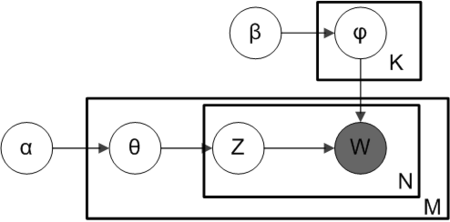
\includegraphics[scale=0.5]{lda.png}
	\caption{LDA plate notation}
\label{fig_lda}
\end{figure}

We mentioned in previous paragraph that our dataset has relatively smaller size compared to common topic model researches. Hence, we assembled various topic models with specialty in short text as suggested by\cite{b6}. The whole list of topic models could be seen in Table~\ref{table 2: topic model experiment} that could be categorized into 4 types. The first type is standard, referred to the baseline topic model which is LDA. The second type, one-topic sampling based, will modify the inference process to sample only one topic per document, meaning all words from a single document will only have one topic label. The third type, global word co-occurrence based, will modify document representation into word-network or set of biterms. Self-aggregation based as the last type will merge several documents into one single pseudo-document and then apply standard-type topic model to it. 

\begin{table}[b]
\renewcommand{\arraystretch}{1.3}
\caption{Topic Model Experiment}
\label{table 2: topic model experiment}
\centering
{\begin{tabular}{|c|P{4.5cm}|c|}
\hline
\textbf{No.}&\textbf{Topic Model}&\textbf{Type}\\
\hline
1&LDA\cite{b8}&Standard  \\
\hline
\multirow{2}{*}{\shortstack{2}}&Dirichlet Multinomial&\multirow{8}{*}{\shortstack{One-topic \\sampling based}} \\
&Mixture (DMM)\cite{b11}&\\\cline{1-2}
3&Latent-Feature LDA (LFLDA)\cite{b12}& \\\cline{1-2}
4&Latent-Feature DMM (LFDMM)\cite{b12}& \\\cline{1-2}
\multirow{2}{*}{\shortstack{5}}&Generalized Polya Urn DMM (GPU-DMM)\cite{b13}& \\\cline{1-2}
\multirow{2}{*}{\shortstack{6}}&GPU Poisson-based DMM (GPU-PDMM)\cite{b14}& \\
\hline
7&Biterm Topic Model (BTM)\cite{b15}&\multirow{3}{*}{\shortstack{Global word \\co-occurence based}} \\\cline{1-2}
\multirow{2}{*}{\shortstack{8}}&Word Network& \\
&Topic Model (WNTM)\cite{b16}&\\
\hline
\multirow{2}{*}{\shortstack{9}}&Self-aggregate&\multirow{3.5}{*}{\shortstack{Self-aggregation \\based}}\\
& Topic Model (SATM)\cite{b17}&\\\cline{1-2}
10&Pseudo-based Topic Model (PTM)\cite{b18}& \\
\hline
\end{tabular}}
\end{table}

After the experiment is done, we will decide what is the best topic model, hyperparameters, and the number of sentence augmentation processes to use. After that, we will incorporate the result to a new background-knowledge-backed topic model called Source-LDA\cite{b9} as the most suitable topic model for our case. In Source-LDA, we can use background knowledge data to influence topic labeling thus improving topic quality in the process.

\subsection{Distribution Similarity}
In this step, we aimed to picture the topic distribution into a single value that describes the rate of consensus built (convergence rate). In order to do this, we used distribution similarity calculation using Jensen-Shannon Divergence across all distributions\cite{b10}. This concludes the final step of our proposed method.

\section{Experiment}
\label{sec_exp}
We had an opportunity to utilize dialog data from requirement decisions (discussion session) of 4 Japanese companies. Firstly, data preprocessing and sentence 
augmentation is done to clean the data. The comparison of dataset characteristics before and after augmentation is shown in Table~\ref{table 3: augmented dataset characteristics}. We managed to expand the dataset up to 1634.46\% from the original size in terms of number of documents, and up to 145.04\% in terms of corpus size. 

\begin{table}[t]
\renewcommand{\arraystretch}{1.3}
\caption{Augmented Dataset Characteristics}
\label{table 3: augmented dataset characteristics}
\centering
{\begin{tabular}{|P{2cm}|P{2cm}|P{1cm}|P{1cm}|}
\hline
\multirow{2}{*}{\shortstack{\textbf{Augmentation}}}&\textbf{Total Documents}&\textbf{Corpus Size}&\textbf{Average Length}\\
\hline
No Augmentation&\multirow{2}{*}{\shortstack{383}}&\multirow{2}{*}{\shortstack{686}}&\multirow{2}{*}{\shortstack{4.83}}\\
\hline
1 Sentence Augmentation&\multirow{2}{*}{\shortstack{1017}}&\multirow{2}{*}{\shortstack{922}}&\multirow{2}{*}{\shortstack{5.00}} \\
\hline
9 Sentence Augmentation&\multirow{2}{*}{\shortstack{5085}}&\multirow{2}{*}{\shortstack{1519}}&\multirow{2}{*}{\shortstack{5.10}} \\
\hline
12 Sentence Augmentation&\multirow{2}{*}{\shortstack{6643}}&\multirow{2}{*}{\shortstack{1681}}&\multirow{2}{*}{\shortstack{5.10}} \\
\hline
\end{tabular}}
\end{table}

Furthermore, the dataset property is presented in Table~\ref{table 4: dataset property}. During dialog data collecting process, 2 types of question were asked. Problem-type question was given at the early stage of discussion while solution-type question is asked at the later stage of discussion. Another property is 'response category' that referred to participant's own division, and 'organization level' that referred to participant's hierarchical  level in the company.

\begin{table}[b]
\renewcommand{\arraystretch}{1.3}
\caption{Dataset Property}
\label{table 4: dataset property}
\centering
{\begin{tabular}{|c|P{5cm}|}
\hline
\textbf{Property Name}&\textbf{Possible value}\\
\hline
Company ID&\{1,2,3,4\}  \\
\hline
Question Type&\{Problem, Solution\} \\
\hline
\multirow{2.5}{*}{\shortstack{Response Category}}&\{Information Technology, Corporate Management, Business Process, Human Development\}\\
\hline
Organization Level&\{very low, low, medium, high, very high\} \\
\hline
Opinion&\{short sentence consists around 5 words\} \\
\hline
\end{tabular}}
\end{table}

Following data preprocessing step, topic model experiment is conducted on all topic models in Table~\ref{table 2: topic model experiment}. We used {\it topic coherence} value to evaluate topic model performance because our dataset is raw and doesn't have any golden labels\cite{b6}. The result of topic model experiment is shown in Fig.~\ref{fig_tme}. The hyperparameter used in this experiment is number of iteration (1000-2000),  $\alpha$ value (0.05-0.3), and  $\beta$ value (0.005-0.03). The number shown in the figure is the average of topic coherence value of all possible hyperparameters for each sentence augmentation processes. Based on the number of sentence augmentation, 9 augmentation is not producing significant result while 1 augmentation gives the best and most consistent result. Self-Augment Topic Model (SATM) gives a good overall score regardless the number of sentence augmentation process. However, LDA held the best score of all experiment with 1 augmentation process. We picked LDA topic model with $\alpha$ value of 0.15, $\beta$ value of 0.01, 2000 iteration, and 1 sentence augmentation process as the best configuration.

\begin{figure}[t]
	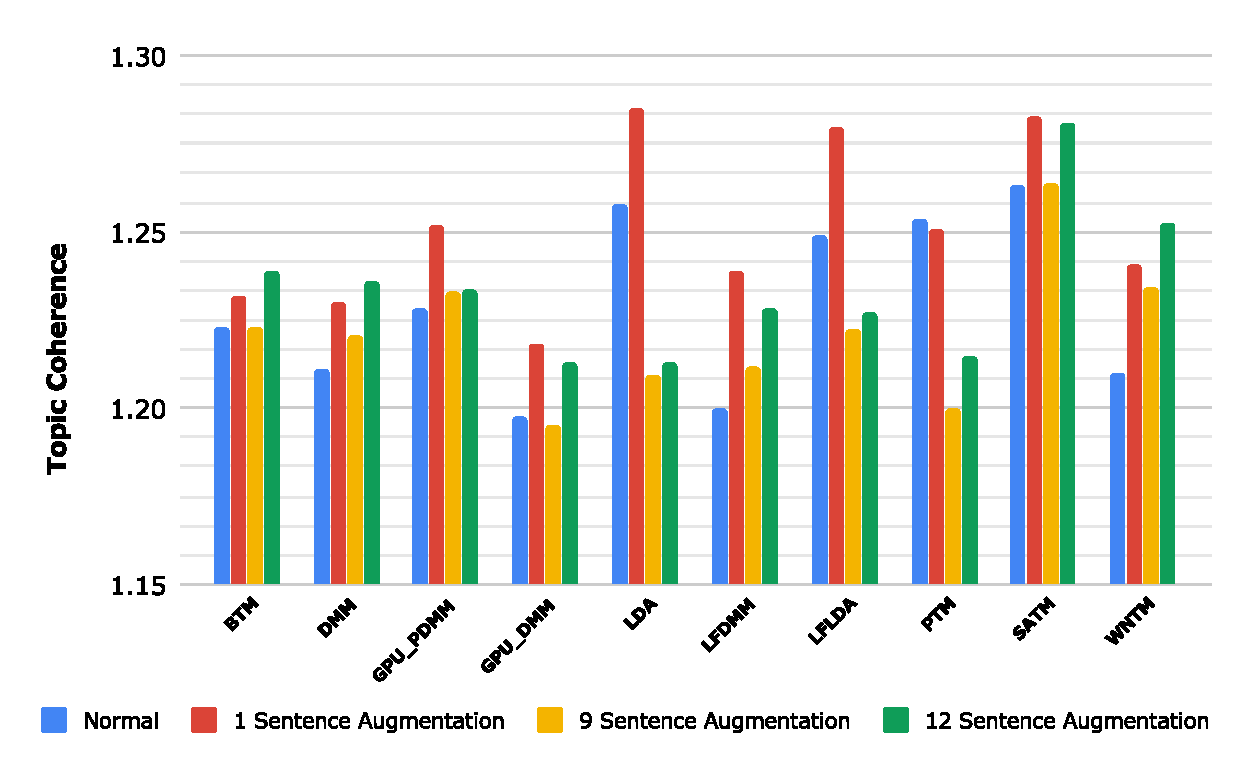
\includegraphics[scale=0.425]{new-topic1.pdf}
	\caption{Topic coherence value based on topic model and sentence augmentation process performed on Dialog Data}
\label{fig_tme}
\end{figure}

The next step is to incorporate the best configuration into  Source-LDA. Based on our proposed method in Section~\ref{sec_pm}, we are using PLM-themed discussion activity as our dataset. Hence, PLM topics is used as the background knowledge data. We decided to use PTC Value Roadmap\footnote{\url{http://support.ptc.com/WCMS/files/28837/en/J1051_ValueRoadmap_TS.pdf}} because it contains many PLM Topics with complete definitions for each topic. The background knowledge dataset held a relatively big size consisting of 26 topics, 1068 unique words, and 145.88 average document length. 

Fig.~\ref{fig_tme2}
\begin{figure}[b]
	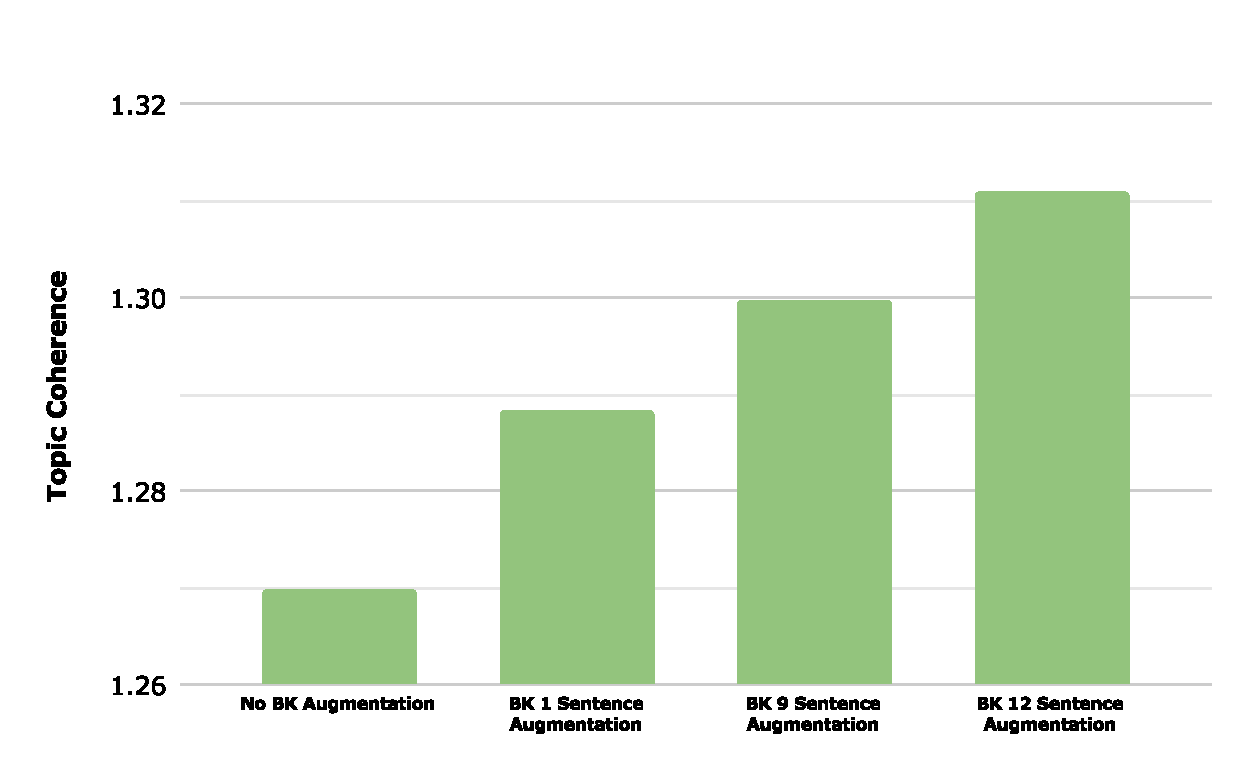
\includegraphics[scale=0.425]{new-topic2.pdf}
	\caption{Topic coherence value based on background knowledge (BK) augmentation process}
\label{fig_tme2}
\end{figure}
shows the topic coherence value relative to the number of sentence augmentation process applied to background knowledge dataset. The topic coherence value is increasing proportionally with the number of sentence augmentation. We only used LDA algorithm because it is the best configuration we conclude from previous paragraph. The usage of sentence augmentation on background knowledge improves topic coherence up to 3.25\%. We picked 12 sentence augmentation process on background knowledge as the best configuration.

The final best configuration we found is by using LDA topic model, $\alpha$ value of 0.15, $\beta$ value of 0.01, 2000 iteration, 1 sentence augmentation on dialog dataset, and 12 sentence augmentation on background knowledge. We are planning to use this finding in future experiment.

\section{Results and Discussion}
In this section, we compared our findings with previous research\cite{b4} as shown in [FIGURE]. We compared between both approaches using topic coherence value with the same dataset and same number of topics. We conclude that the usage of data augmentation and background knowledge will gives a better result.



Furthermore, we applied the best configuration stated in Section~\ref{sec_exp} to create topic distributions of the dataset. Then, we calculate the convergence rate among topic distributions and do qualitative evaluation together with external facilitator. 

During topic modeling process, we replaced background knowledge's topic name with its topic number to increase readability. The mapping of topic number with its actual name can be seen at Table~\ref{table 5: mapping plm} with a side note that the order of topic number is in alphabetical order and different with what shown in the reference (PTC Value Roadmap). There are 26 PLM Topics in total that serves as best practice for a specific business unit.

\begin{table}[t]
\renewcommand{\arraystretch}{1.3}
\caption{Mapping of PLM Topics}
\label{table 5: mapping plm}
\centering
{\begin{tabular}{|c|c|}
\hline
\textbf{Topic No.}&\textbf{PLM Topics}\\
\hline
Topic 0&Business System Support  \\
\hline
Topic 1&Change and Configuration Management \\
\hline
Topic 2&Component and Supplier Management \\
\hline
Topic 3&Concept Development \\
\hline
Topic 4&Design and Manufacturing Outsourcing \\
\hline
\multirow{2}{*}{Topic 5}&Equipment Monitoring and\\
&Lifecycle Management \\
\hline
Topic 6&Manufacturing Process Management \\
\hline
\multirow{2}{*}{Topic 7}&Mechanical, Electrical, and \\
&Software Development \\
\hline
Topic 8&Performance Analysis and Feedback \\
\hline
Topic 9&Platform Design and Variant Generation \\
\hline
Topic 10&Product Cost Management \\
\hline
Topic 11&Product Support Analysis and Planning \\
\hline
Topic 12&Project Management \\
\hline
Topic 13&Quality and Reliability Management \\
\hline
Topic 14&Regulatory and Materials Compliance \\
\hline
Topic 15&Requirements Definition and Management \\
\hline
Topic 16&Service Diagnostics and Knowledge Management \\
\hline
\multirow{2}{*}{Topic 17}&Service Logistics and\\
&Network Management \\
\hline
\multirow{2}{*}{Topic 18}&Service Order Management and\\
&Field Service \\
\hline
Topic 19&Service Parts Planning and Pricing \\
\hline
Topic 20&Smart, Connected Product Enablement \\
\hline
Topic 21&System Architecture Design \\
\hline
\multirow{2}{*}{Topic 22}&Technical and Service Parts \\
&Information Creation and Delivery\\
\hline
Topic 23&Tooling Design and Manufacture \\
\hline
Topic 24&Verification and Validation \\
\hline
\multirow{2}{*}{Topic 25}&Warranty and Performance-based \\
&Contract Management\\
\hline
\end{tabular}}
\end{table}

The average topic distribution of sentences in dialog data from each company is shown in Fig.~\ref{fig_c}. The most probable and least probable topic is different for each company. For example, company 1 that runs in business process innovation industry discussed a lot about topic \#12 (Project Management) and very little about topic \#24 (Verification and Validation). Meanwhile, Company 2 from automotive manufacturer industry had a huge interest in topic \#18 (Service Order Management and Field Service) but not in topic \#22 (Technical and Service Parts Information Creation and Delivery). Company 3 from aqua industry has topic \#19 (Service Parts Planning and Pricing) as the most probable topic and topic \#2 (Component and Supplier Management) as the least probable topic. Lastly, company 4 from automotive supplier industry had topic \#22 and topic \#21 (System Architecture Design) as their most probable topics.


% An example of a floating table. Note that, for IEEE style tables, the 
% \caption command should come BEFORE the table. Table text will default to
% \footnotesize as IEEE normally uses this smaller font for tables.
% The \label must come after \caption as always.
%
%\begin{table}[!t]
%% increase table row spacing, adjust to taste
%\renewcommand{\arraystretch}{1.3}
% if using array.sty, it might be a good idea to tweak the value of
% \extrarowheight as needed to properly center the text within the cells
%\caption{An Example of a Table}
%\label{table_example}
%\centering
%% Some packages, such as MDW tools, offer better commands for making tables
%% than the plain LaTeX2e tabular which is used here.
%\begin{tabular}{|c||c|}
%\hline
%One & Two\\
%\hline
%Three & Four\\
%\hline
%\end{tabular}
%\end{table}

Given the topic distributions, we will conduct similarity measurement using JS Divergence to find convergence rate. The interpretation value of JS divergence ranges from 0-1. All value approaching to 0 means that there is no variation between probability distributions, meanwhile value approaching to 1 means that there is high variation between probability distributions. The convergence of each discussion sessions can be seen at Table~\ref{table 6: similarity} along with the top frequent words. The overall convergence rate achieved from each discussion is probably not too good since each one has convergence rate above 0.500. The lowest degree of convergence was achieved by Company 1 with 0.865 while the highest degree of convergence was achieved by Company 3 with 0.672.  The top words from each discussion acts as a support to better understand the discussion.

Given the results, here is the feedback from professional consultant for each discussion session:
\medskip

\subsubsection{Company 1}
{\it Company 1 had a key problem in terms of information exchange between design and manufacturing. I agree that the frequency of Design and Manufacturing topics was high. However, the topic of Project Management was rarely spoken directly by their voices. In addition, the analysis results show that there are few topics on Manufacturing Process Management. Certainly, there were few remarks on Manufacturing Process Management when the workshop was actually held. However, one of the participants was very concerned about the topic and he is one of the important people in the PLM project, so even if it is a minority opinions, I cannot ignore it as my consultant perspective. By the way, in the analysis results, the words with the highest frequency of occurrence were Information, Product, and Data. These were key words that participants often talked about during the actual workshop. As a consultant, I agree with that.}
\smallskip

\subsubsection{Company 2}
{\it The company 2 had three business unit. Thus, the participants had different opinions, as each business unit had a completely different product and each business model was different. When I looked at the results of this analysis, I thought that the reason that the topic of Verification and Validation was high was probably that they had a problem with their product quality. However, although the topic about Field Service has not been talked about in the actual workshop time, the frequency of topic 18 was high in this analysis result. In fact, this company does little field service work, so it is necessary to confirm why such analysis results were performed. In addition, the analysis results indicated that the frequency of Product Cost Management and Project Management topics was low. However, I think the discussions about costs and projects were relatively common during the actual discussions with them. Regarding the word distribution, the analysis result, it showed that the frequency of Production, Work, and Product were high. I agree with this result.}
\smallskip

\subsubsection{Company 3}
{\it The motivation for Company 3 to introduce PLM was to strengthen its field service operations. Looking at the analysis results, it was found that the topics with the highest frequency were field services, such as Warranty management, Performance Based Contract Management, Technical Service Parts Information, and Service Order Management. I agree this result as a professional consultant. However, regarding the monitoring and management of equipment, it was analyzed that the topic frequency was low. This is different from the actual situation, because in the actual workshop, the story of equipment monitoring was relatively well discussed. The frequency of words of Resource, Human, Product, and Development is high. Even during the actual workshop discussion, the shortage of human resources in field service was very problematic. Thus, I agree with the analysis results.}
\smallskip

\begin{figure*}[t]
	\subfloat[Topic distributions for company 1]{\label{fig_c1}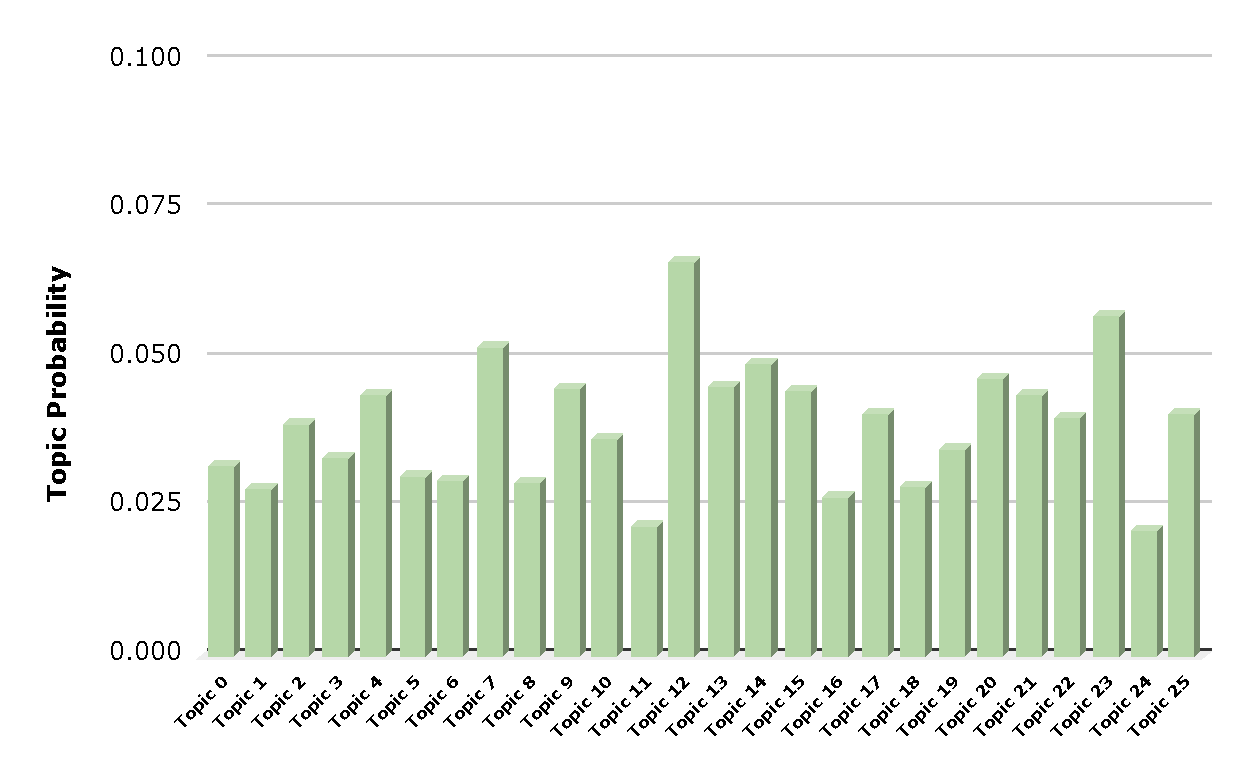
\includegraphics[scale=0.425]{new-company1.pdf}}
	\subfloat[Topic distributions for company 2]{\label{fig_c2}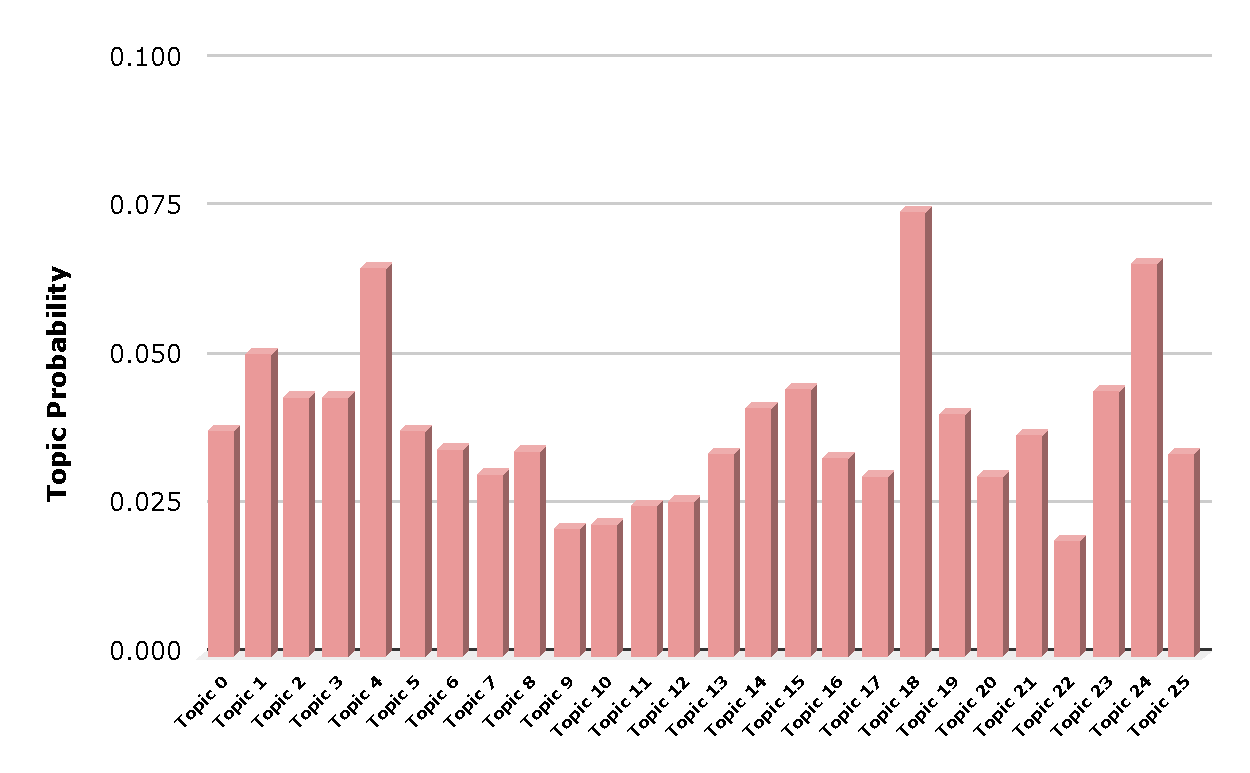
\includegraphics[scale=0.425]{new-company2.pdf}}\\
	\subfloat[Topic distributions for company 3]{\label{fig_c3}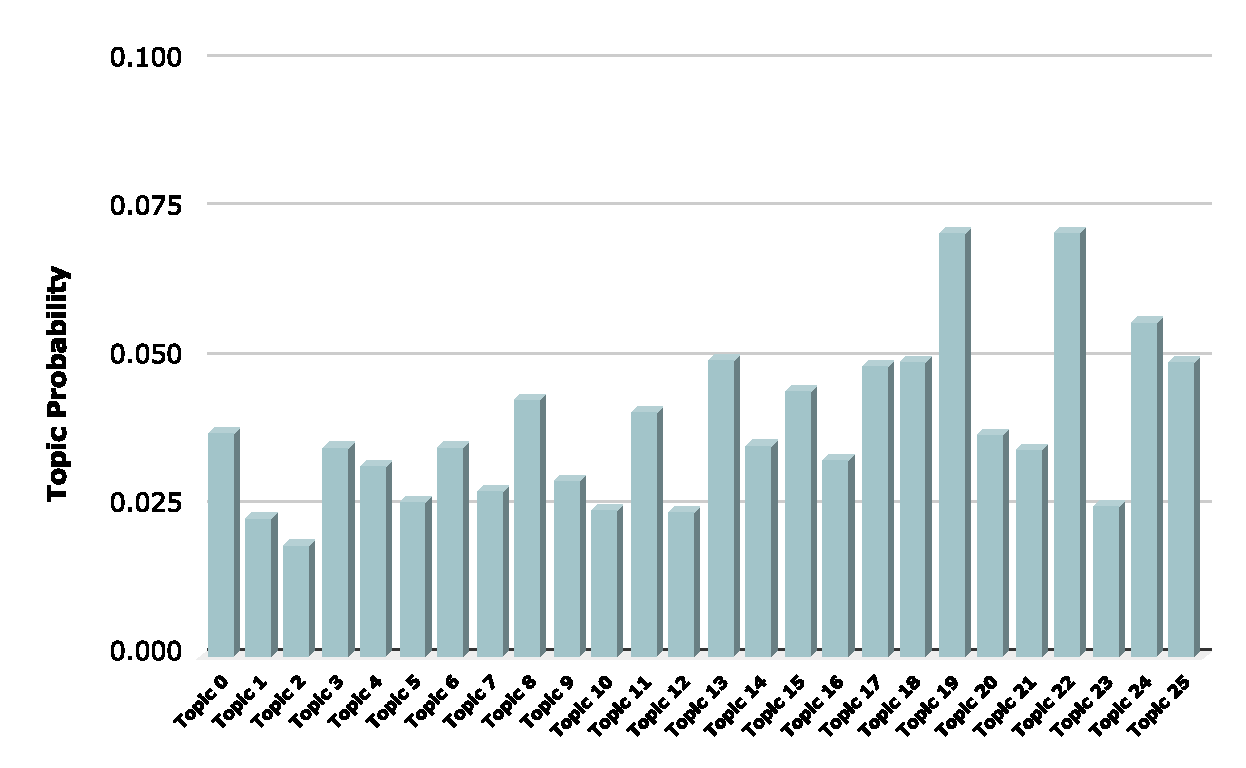
\includegraphics[scale=0.425]{new-company3.pdf}}
	\subfloat[Topic distributions for company 4]{\label{fig_c4}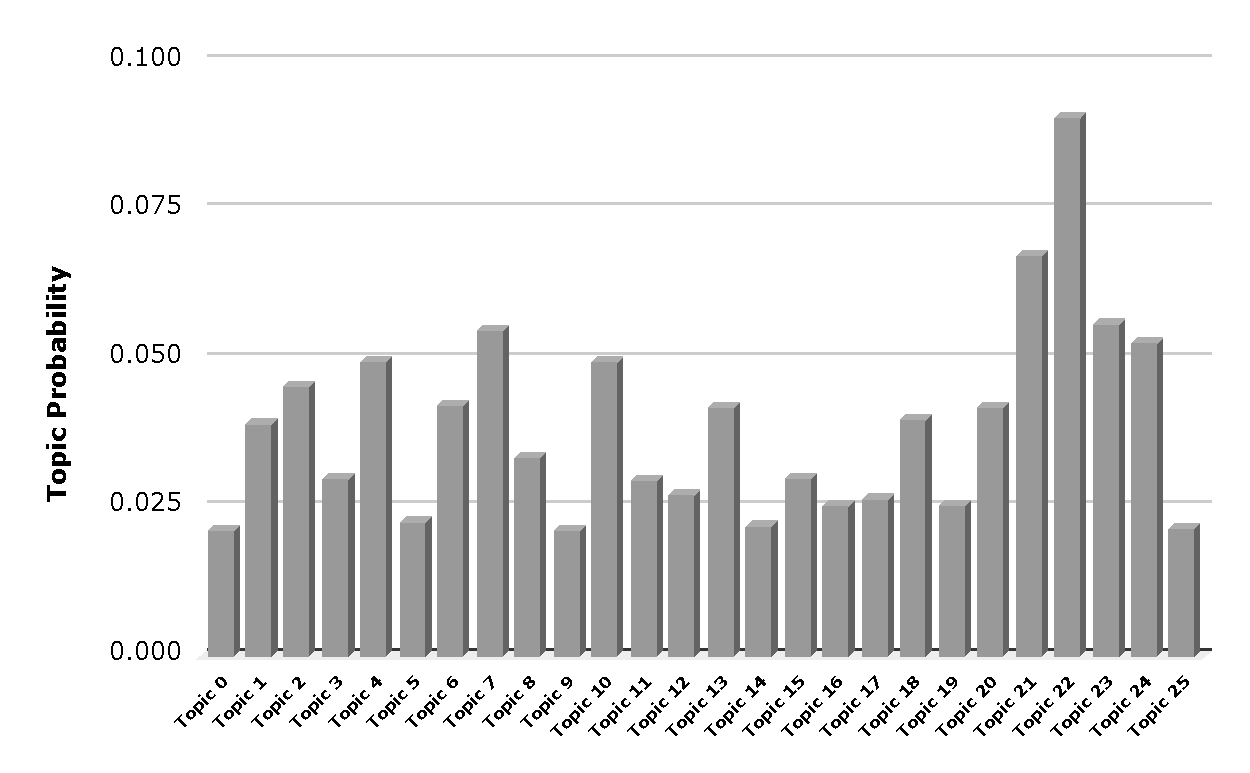
\includegraphics[scale=0.425]{new-company4.pdf}}
\caption{Average topic distributions of sentences in dialog data of all company}
\label{fig_c}
\end{figure*}

\subsubsection{Company 4}
{\it Company 4 has been practicing efforts to make its factory a smart factory. As a consultant, what I noticed in their actual workshops was their lack of information sharing between departments and insufficient training of employees. On the other hand, looking at the results of this analysis, we found that the topic \# 22 was Technical and Service Part Information Creation and Delivery. At first, I wasn't interested in topic \# 22. However, after reviewing the content of discussions with the workshop participants at a later date, there was an opinion that attention was paid to the management of service parts in order to contribute to sustainable sales. It seems that the results of this analysis have taught me a topic that I did not notice at first. Looking at the analysis results of the word distribution, it seems that three words, Information, Data, and Sharing, appear frequently. This was exactly the issue that was being talked about at the workshop. Additionally, The analysis results seem to indicate that there is no relationship between education and system design. Further investigation is needed as I think education topic should be highly related in the workshop.}
\medskip

\begin{table}[b]
\renewcommand{\arraystretch}{1.3}
\caption{Convergence Rate and Top Words}
\label{table 6: similarity}
\centering
{\begin{tabular}{|c|c|P{3.5cm}|}
\hline
\textbf{Company ID}&\textbf{Convergence Rate}&\textbf{Top words}\\
\hline
Company 1&0.865&\{Information, Product, Data\}  \\
\hline
Company 2&0.766&\{Production, Work, Product\} \\
\hline
\multirow{2}{*}{\shortstack{Company 3}}&\multirow{2}{*}{\shortstack{0.672}}&\{Resource, Human, Product, Development\} \\
\hline
Company 4&0.753&\{Information, Data, Sharing\} \\
\hline
\end{tabular}}
\end{table}


Based on our analysis and feedback from professional consultant. We feel that our experiment on the usage of topic model with background knowledge in an industrial engineering discussion activity (in this case, PLM-themed) gives an actual contribution towards discussion summarization in which, might improve consensus building process. The important takeaway of this  research is that topic modeling with background knowledge will assist professional consultant to understand more towards participant's latent opinion.

\section{Conclusion and Future Works}
In this paper, we analysed a new digitized approach to improve consensus building process in discussion activity held within industrial engineering context (PLM-themed). Our proposed method consists of performing data augmentation, implementing topic model with background knowledge, and calculating the distribution similarity. Finally, we validate the result on professional consultant. We received good feedback which validates our purpose of using a new approach to improve consensus building process. Moreover, we also found that using data augmentation and background knowledge in topic modeling will improve its topic quality.

However, further approach is still necessary based on two perspective: consensus building and topic modeling. From consensus building perspective, we still need to assure the emotional state of discussion participants when dialog data is recorded. Some variables might aspect the quality and consistency of participant's opinion. Meanwhile from topic modeling perspective, we are planning to expand Source-LDA so it can afford different data representation like BTM and WNTM does.

% An example of a floating figure using the graphicx package.
% Note that \label must occur AFTER (or within) \caption.
% For figures, \caption should occur after the \includegraphics.
% Note that IEEEtran v1.7 and later has special internal code that
% is designed to preserve the operation of \label within \caption
% even when the captionsoff option is in effect. However, because
% of issues like this, it may be the safest practice to put all your
% \label just after \caption rather than within \caption{}.
%
% Reminder: the "draftcls" or "draftclsnofoot", not "draft", class
% option should be used if it is desired that the figures are to be
% displayed while in draft mode.
%
%\begin{figure}[!t]
%\centering
%\includegraphics[width=2.5in]{myfigure}
% where an .eps filename suffix will be assumed under latex, 
% and a .pdf suffix will be assumed for pdflatex; or what has been declared
% via \DeclareGraphicsExtensions.
%\caption{Simulation Results}
%\label{fig_sim}
%\end{figure}

% Note that IEEE typically puts floats only at the top, even when this
% results in a large percentage of a column being occupied by floats.


% An example of a double column floating figure using two subfigures.
% (The subfig.sty package must be loaded for this to work.)
% The subfigure \label commands are set within each subfloat command, the
% \label for the overall figure must come after \caption.
% \hfil must be used as a separator to get equal spacing.
% The subfigure.sty package works much the same way, except \subfigure is
% used instead of \subfloat.
%
%\begin{figure*}[!t]
%\centerline{\subfloat[Case I]\includegraphics[width=2.5in]{subfigcase1}%
%\label{fig_first_case}}
%\hfil
%\subfloat[Case II]{\includegraphics[width=2.5in]{subfigcase2}%
%\label{fig_second_case}}}
%\caption{Simulation results}
%\label{fig_sim}
%\end{figure*}
%
% Note that often IEEE papers with subfigures do not employ subfigure
% captions (using the optional argument to \subfloat), but instead will
% reference/describe all of them (a), (b), etc., within the main caption.


% Note that IEEE does not put floats in the very first column - or typically
% anywhere on the first page for that matter. Also, in-text middle ("here")
% positioning is not used. Most IEEE journals/conferences use top floats
% exclusively. Note that, LaTeX2e, unlike IEEE journals/conferences, places
% footnotes above bottom floats. This can be corrected via the \fnbelowfloat
% command of the stfloats package.



%\section{Conclusion}
%The conclusion goes here. this is more of the %conclusion

% conference papers do not normally have an appendix


% use section* for acknowledgement
%\section*{Acknowledgment}


%The authors would like to thank...
%more thanks here


% trigger a \newpage just before the given reference
% number - used to balance the columns on the last page
% adjust value as needed - may need to be readjusted if
% the document is modified later
%\IEEEtriggeratref{8}
% The "triggered" command can be changed if desired:
%\IEEEtriggercmd{\enlargethispage{-5in}}

% references section

% can use a bibliography generated by BibTeX as a .bbl file
% BibTeX documentation can be easily obtained at:
% http://www.ctan.org/tex-archive/biblio/bibtex/contrib/doc/
% The IEEEtran BibTeX style support page is at:
% http://www.michaelshell.org/tex/ieeetran/bibtex/
%\bibliographystyle{IEEEtran}
% argument is your BibTeX string definitions and bibliography database(s)
%\bibliography{IEEEabrv,../bib/paper}
%
% <OR> manually copy in the resultant .bbl file
% set second argument of \begin to the number of references
% (used to reserve space for the reference number labels box)
\begin{thebibliography}{1}
  
\bibitem{b1} J.~Thomas-Lamar, S.~Mckearnan, and L.~Susskind, \emph{The consensus building handbook: a comprehensive guide to reaching agreement}. \hskip 1em plus
  0.5em minus 0.4em\relax SAGE Publications, 1999. pp. 7--9.
 
\bibitem{b23} J.~Stark, \emph{Product lifecycle management}. \hskip 1em plus
 0.5em minus 0.4em \relax Springer, 2015.
 
\bibitem{b2} N.~He, S.~Yao, and O.~Yoshie, \emph{Emotional speech classification in consensus building}. \hskip 1em plus
  0.5em minus 0.4em\relax 2014 10th International Conference on Communications (COMM), Bucharest, 2014, pp. 1-4.
  
\bibitem{b3} S.~Goto, O.~Yoshie, and S.~Fujimura, \emph{Preliminary Study: Text mining approach to dialog data of stakeholders on requirement decision for Enterprise Information System}. \hskip 1em plus
  0.5em minus 0.4em\relax 2019 10th Annual European Decision Sciences Institute (EDSI) Conference, Nottingham, 2019.

\bibitem{b24} C.~H. Matt and A.~Benlian, \emph{Digital transformation strategies}. \hskip 1em plus
  0.5em minus 0.4em\relax Business \& Information Systems Engineering Vol. 57, 2015, pp. 339-343.

\bibitem{b4} S.~Goto, O.~Yoshie, and S.~Fujimura, \emph{Empirical study of multi-party workshop facilitation in strategy planning phase for Product Lifecycle Management (PLM) system}. \hskip 1em plus
  0.5em minus 0.4em\relax 2019 International Federation for Information Processing (IFIP) International Conference on Product Lifecycle Management, Moscow, 2019, pp. 82-93.

\bibitem{b5} Y.~Katagiri et al., \emph{Implicit proposal filtering in multi-party consensus-building conversations}. \hskip 1em plus
  0.5em minus 0.4em\relax Proceedings of the 9th SIGdial Workshop on Discourse and Dialogue, Columbus, 2008, pp. 100-103.

\bibitem{b20} C.~T. L. Butler and A.~Rothstein, \emph{On conflict and consensus; A handbook on formal consesus decision making}. \hskip 1em plus
  0.5em minus 0.4em\relax Food Not Bombs Publishing, Takoma Park, 2004.

\bibitem{b21} R.~O. Briggs, G.~Kolfschoten, and G.~J. de Vreede, \emph{Toward a theoretical model of consensus building}. \hskip 1em plus
  0.5em minus 0.4em\relax  11th Americas Conference on Information Systems, 2005.

\bibitem{b22} M.~M. Shepherd and W.~B. Martz Jr, \emph{Group consensus: Do we know it when we see it?} \hskip 1em plus
  0.5em minus 0.4em\relax Proceedings of the Hawaii International Conference on System Science, Los Alamitos, 2004.

\bibitem{b6} J.~Qiang, Z.~Qian, Y.~Li, Y.~Yuan, and X.~Wu, \emph{Short text topic modeling techniques, applications, and performance: a survey}. \hskip 1em plus
  0.5em minus 0.4em\relax 2019.

\bibitem{b7} J.~Wei and K.~Zou, \emph{EDA: Easy Data Augmentation techniques for boosting performance on text classification tasks}. \hskip 1em plus
  0.5em minus 0.4em\relax Proceedings of the 2019 Conference on Empirical Methods in Natural Language Processing and the 9th International Joint Conference on Natural Language Processing (EMNLP-IJCNLP), Hong Kong, 2019, pp. 6383-6389.

\bibitem{b8} D.~M. Blei, A.~Y. Ng, and M.~I. Jordan, \emph{Latent Dirichlet Allocation}.\hskip 1em plus
  0.5em minus 0.4em\relax Proceedings of the 14th International Conference on Neural Information Processing Systems: Natural and Synthetic, Vancouver, 2001, pp. 601-608.

\bibitem{b9} J.~Wood, P.~Tan, W.~Wang, and C.~Arnold, \emph{Source-LDA: Enhancing probabilistic topic models using prior knowledge sources}. \hskip 1em plus
  0.5em minus 0.4em\relax 33rd IEEE International Conference on Data Engineering (ICDE), San Diego, 2017, pp. 411-422. 

\bibitem{b10} J.~A. Aslam and V.~Pavlu, \emph{Query hardness estimation using Jensen-Shannon Divergence among multiple scoring functions}. \hskip 1em plus
  0.5em minus 0.4em\relax 29th European Conference on Information Retrieval Research (ECIR), Rome, 2007, pp. 198-209.

\bibitem{b11} J.~Yin and J.~Wang, \emph{A dirichlet multinomial mixture model-based approach for short text clustering}. \hskip 1em plus
  0.5em minus 0.4em\relax Proceedings of the 20th ACM SIGKDD International Conference on Knowledge Discovery and Data Mining, New York,2014, pp. 233-242.

\bibitem{b12} D.~Q. Nyugen, R.~Billingsley, L.~Du, and M.~Johnson, \emph{Improving topic models with latent feature word representations}. \hskip 1em plus
  0.5em minus 0.4em\relax Transactions of the Association for Computational Linguistics vol. 3, 2015, pp. 299-313.

\bibitem{b13} C.~Li et al., \emph{Topic modeling for short texts with auxiliary word embeddings}. \hskip 1em plus
  0.5em minus 0.4em\relax Proceedings of the 39th International ACM SIGIR Conference on Research and Development in Information Retrieval, Pisa, 2016, pp. 165-174.

\bibitem{b14} C.~Li et al., \emph{Enhancing topic modeling for short texts with auxiliary word embeddings}. \hskip 1em plus
  0.5em minus 0.4em\relax ACM Transactions on Information Systems (TOIS), 2017, pp. 1-30.

\bibitem{b15} X.~Cheng, X.~Yan, Y.~Lan, and J.~Guo, \emph{Btm: Topic modeling over short texts}. \hskip 1em plus
  0.5em minus 0.4em\relax IEEE Transactions on Knowledge and Data Engineering, 2014, pp. 2928-2941.

\bibitem{b16} Y.~Zuo, J.~Zhao, and K.~Xu, \emph{Word network topic model: a simple but general solution for short and imbalanced texts}. \hskip 1em plus
  0.5em minus 0.4em\relax Knowledge and Information Systems, 2016, pp. 379-398.

\bibitem{b17} X.~Quan, C.~Kit, Y.~Ge, and S.~J. Pan, \emph{Short and sparse text topic modeling via self-aggregation}. \hskip 1em plus
  0.5em minus 0.4em\relax Proceedings of the 24th International Conference on Artificial Intelligence, Buenos Aires, 2015, pp. 2270-2276.

\bibitem{b18} Y.~Zuo et al., \emph{Topic modeling of short texts: A pseudo-document view}. \hskip 1em plus
  0.5em minus 0.4em\relax Proceedings of the 22nd ACM SIGKDD international conference on knowledge discovery and data mining, San Fransisco, 2016, pp. 2105-2114.

\bibitem{b19} K.~Ondrej and J.~Marlin, \emph{Product life cycle in digital factory}. \hskip 1em plus
  0.5em minus 0.4em\relax Knowledge management and innovation: a business competitive edge perspective, Cairo, 2010, pp. 1881-1886.  

\end{thebibliography}

\appendix[Preliminary Experiment]
\label{appendix_1}
\noindent We conduct a preliminary experiment to prove the effectiveness of our method. The dialog data we used is an original data with very limited context and small corpus size. Hence, we would like to validate our method by experimenting it on a widely used dataset. We performed data augmentation processes on Biomedical dataset taken from\cite{b6} which has 20 topics, 4498 corpus, 19448 documents, and 7.44 average document length. Then, we perform topic modeling using LDA, BTM, and PTM algorithm. Finally, we evaluate it by calculating their topic coherence value. Fig.~\ref{fig_tmv} shows that data augmentation will improve topic quality on a certain degree.

\begin{figure} [H]
	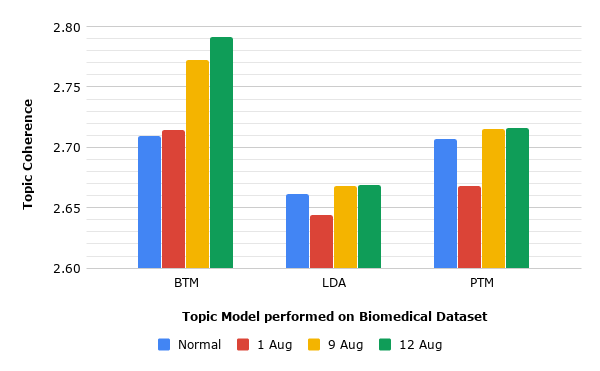
\includegraphics[scale=0.425]{topic3.png}
	\caption{Topic coherence value based on topic model and sentence augmentation process performed on Biomedical Dataset}
\label{fig_tmv}
\end{figure}


% that's all folks
\end{document}


